
\section{Experimental Tools}\label{method:tools}

In order to explore the large number of possible exchange instances described in
\S \ref{method:setup}, a sophisticated problem solving framework is needed. This
section describes the design principles and implementation details of a new
software package called Cyclopts (\underline{Cycl}us \underline{Opt}imization
\underline{S}tudies). Cyclopts, written primarily in Python with a C++ layer
used to operate with Cyclus, provides a general framework for sampling a
parameter space, defining problem instances for a given point in parameter
space, and solving a problem instance under a variety of conditions.

The section begins with a short discussion on terminology in \S
\ref{method:tools:term}.  \S \ref{method:tools:struc} describes the general
Cyclopts workflow and specific features used in the DRE experimental
campaign. \S \ref{method:tools:hdf5} discusses Cyclopts persistence mechanisms,
including database design and layout. The section concludes with \S
\ref{method:tools:htc}, describing Cyclopts' high throughput computing (HTC)
capability, which enables scalable, concurrent execution.

\subsection{Terminology}\label{method:tools:term}

Cyclopts supports a two-tier definition of problem instances, borrowing terms
from biological classification. Problem \textit{families} describe a general
form of problem instance. For example, the Traveling Salesman Problem (TSP)
could be implemented as a problem family. In this analysis, the NFCTP is
considered the problem family, since any given instance of the NFCTP will have
the same general structure. Whether or not the LP or MILP formulation is used is
dependent on whether or not arcs in the Exchange Graph are labeled as exclusive
or not. If there are no exclusive arcs, the LP formulation is used; otherwise,
the MILP formulation is used.

Each problem family can have any number of \textit{species}. One can
conceptualize the relationship as a tree structure, in which families are parent
nodes and species are child nodes. A problem species defines the methodology for
generating \textit{instances} of a problem family. Using the TSP example above,
a problem species may be ``the greater Atlanta metropolitan area'', for which
the effect of regional gas prices may be studied. For the NFCTP study, front-end
and back-end exchanges form two separate species. Each species can have unique
parameters in addition to family-related parameters, is the case for the two
species studied.

\subsection{Design}\label{method:tools:struc}

The full Cyclopts stack is comprised of three phases: generation of parameter
space, generation of instances, and execution of instances. The workflow begins
with user input detailing a range of values for a set of parameters. Cyclopts
then translates the input into a parameter space by enumerating all possible
combinations of parameters. For example, if parameters $x$ and $y$ have defined
values of $[1, 2]$ and $[3, 4, 5]$, respectively, Cyclopts will generate a
parameter space comprised of six points in $(x, y)$ notation: $(1, 3)$, $(1,
4)$, $(1, 5)$, $(2, 3)$, $(2, 4)$, and $(2, 5)$. Each point is then then
provided to a problem species in order to generate one or more problem
instances. Species are expected to define defaults for all parameters as user
input may define values for only a subset of available parameters.

Given a point in parameter space, an instance can be generated. If there are any
stochastic effects during instance generation, many instances may be
generated. Again, because parameters are species dependent, the logic of
instance generation from a set of parameters is the task of a problem
species. Following instance generation, instances may be executed. Cyclopts
supports multiple solution options by design. The same instance may be solved
with both a heuristic and a full optimization solver, for example. Once an
instance of a problem is defined, it is independent of any species-level
effects. Accordingly, instance execution and related logic is the domain of
problem families. 

A summary of the high-level Cyclopts workflow and entities is presented in
Figure \ref{fig:lopts_desgin}. Note that objects generated as the workflow moves
from parameter space to instance solution form a tree structure.

\TODO{update fig}
\begin{figure}
  \begin{center}
    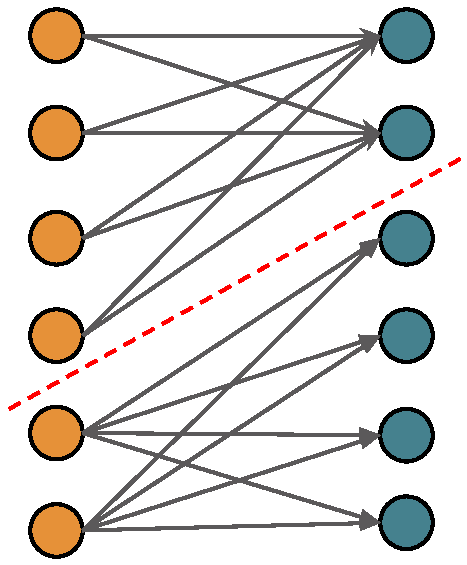
\includegraphics[width=0.55\textwidth]{exchange_part_supreq.pdf}
    \caption[]{
      \label{fig:lopts_desgin}
      Foo.}
  \end{center}
\end{figure}

\subsection{Persistence Mechanisms}\label{method:tools:hdf5}

While the root node in Figure \ref{fig:lopts_desgin} is generated from a
user-provided input file, each subsequent level in the hierarchy represents a
stateful object: a point in parameter space, a problem instance, and a
solution. Each stateful object can be written to and read from disc. Cyclopts
also incorporates a post-processing step, during which all related objects may
be analyzed and aggregate data may be collected and written to disc. While any
input/output (I/O) persistence mechanism is valid, Cyclopts is currently
implemented using Hierarchical Datat Format 5 (HDF5) \cite{hdf5} via PyTables
\cite{pytables}.

Data in HDF5 is stored hierarchicaly, similar to a filesystem. At the root node
of the filesystem-like structure, a \textit{group} is defined for problem family
and problem species data, named \code{Family} and \code{Species},
respectively. A \textit{dataset} for aggregate results named \code{Results} is
also defined. A path in HDF5 is designated in a UNIX-like manner. For example,
the path to \code{Family} would be \code{/Family}, indicating that the group is
directly under the root node, \code{/}. Further, groups are defined for each
kind of family and species. The DRE problem family records data in the group
\code{/Family/ResourceExchange}, front-end exchanges record data in the group
\code{/Species/StructuredRequest}, and back-end exchanges record data in the
group \code{/Species/StructuredSupply}. 

Each stateful object is given a Universally Unique Identifier (UUID) by which it
can be identified for future reading and analysis. The UUID is used in two
distinct capacities: as a \textit{primary key} in a dataset for future
identification or as the name of a group. Whether to aggregate data in one large
dataset or divide data into datasets for each object is a design decision
informed by practical performance. A study of the tradeoffs between each
approach is presented in \S \ref{method:tools:hdf5:study}. As a result of that
study, for objects that are both read and written, the latter approach is taken.

A description of all data gathered for each family and species for convesion,
execution, and postprocessing is rather detailed. Accordingly, Appedix
\ref{app:hdf5} contains all relevant information.

\subsubsection{Performance Studies}\label{method:tools:hdf5:study}

\textit{Chunk size} is a critical parameter of HDF5 datasets that affects I/O
performance. HDF5's storage layout is not contiguous, rather, data is separated
into equal-sized \textit{chunks}. Any reading or writing occurs on a chunk of
data, rather than accesing an entire dataset. Accordingly, choosing a reasonable
chunk size can greatly increase performance for known data access operations. In
PyTables, the \textit{compresison level} of a dataset is also a tuneable
parameter that affects I/O performance. Compression, of course, reduces overall
database size. Therefore, an ideal compression is the largest possible that
retains acceptable performance.

Originally, all Cyclopts datasets used a UUID-as-primary-key layout. For
instance, rather than many tables with a layout described in Table
\ref{tbl:/Family/ResourceExchange/ExchangeArcs},
all related tables were combined and included an extra column naming the
instance UUID. However, extremely long read times were encountered when post
processing data. The basic procedure for performing a post-process operation
included reading all rows associated with a UUID in an input exchange family
dataset, reading all rows associated with the same UUID in an output exchange
species dataset, selecting a value from each row, and performing a dot product
of the resulting vectors.

In order to investigate possible chunk size and compression optimizations, a
small ($\sim$ MBs) dataset and a large ($\sim$ GBs) dataset were created. The
postprocessing step was then run on 25 instances in each dataset. The operation
was timed using the UNIX \code{time} command. Poor performance was experience
with an initial chunksize proportional to the ratio of a normal L2 cache to row
size was used for each dataset and a compression level of four was selected per
suggestions from the PyTables documentation \cite{tablesopt}. Accordingly, chunk
size and compression level were varied around these recommended values in order
to determine if any tuning was available. The results of the study on the small
dataset is shown in Figure \ref{fig:small_db}. The large dataset results is
shown in Figure \ref{fig:large_db}.

\begin{figure}
  \begin{center}
    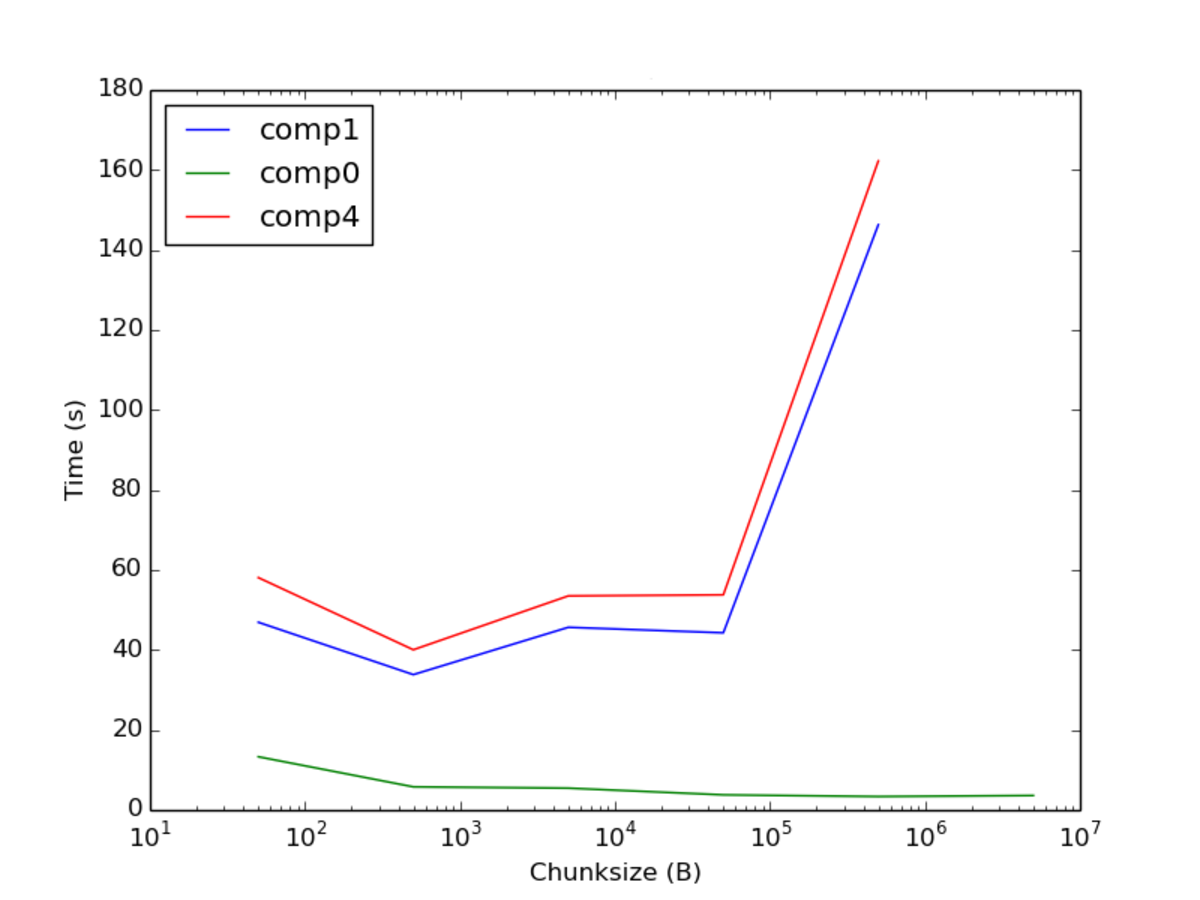
\includegraphics[width=0.85\textwidth]{small_all.pdf}
    \caption[]{
      \label{fig:small_db}
      Postprocessing performance for 25 entries of a small-sized database for a 
      variety of compression levels and chunk sizes.}
  \end{center}
\end{figure}

\begin{figure}
  \begin{center}
    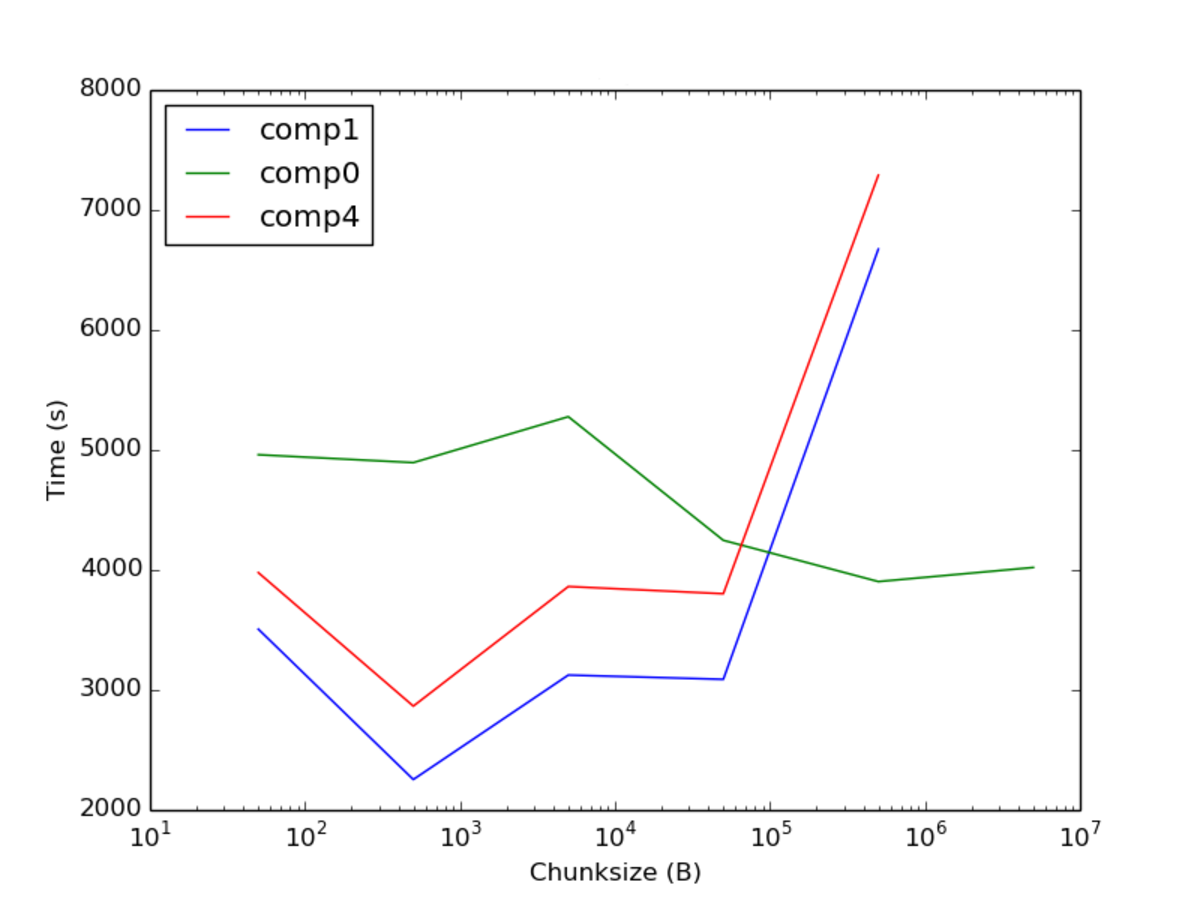
\includegraphics[width=0.85\textwidth]{large_all.pdf}
    \caption[]{
      \label{fig:large_db}
      Postprocessing performance for 25 entries of a large-sized database for a
      variety of compression levels and chunk sizes.}
  \end{center}
\end{figure}

Assuming some level of compression, an ideal chunksize range is identified for
the small database of between $\sim 10^3 - 10^5$ bytes. Further the small
database example confirms that the study's methodology is well founded: an ideal
chunksize range is established. A similar optimal chunk size range is found for
the large database. However, note that in this exercise, only $\sim 0.25\%$ of
instances are postprocessed. An optimal performance of $> 80$ seconds per
instance is unacceptable.

A number of strategies exist for trying to increase performance. A classic
strategy is pivoting the group-dataset structure such that data queries are made
upon a group rather than rows in a dataset. In this example, such a pivot
involves dividing the single, large dataset into $n$ datasets, where $n$ is the
number of unique primary keys (UUIDs in this case). 

Accordingly, an additional test was conducted such that all datasets on which
queries are made were pivoted such that new group nodes were added for each
UUID, and all data for that UUID was appended to a dataset under the associated
group. The post processing step was divided into the read operations associated
with the exchange family and the the read operations associated with a
species. The exact same operations were then tested on a large database with the
column-based layout and a large database with the group-based layout. Specific
instances, increasing in size, were identified to be postprocessed. The
group-based results were compared with the column-based results and are shown in
Figure \ref{fig:col_grp}.

\begin{figure}
  \begin{center}
    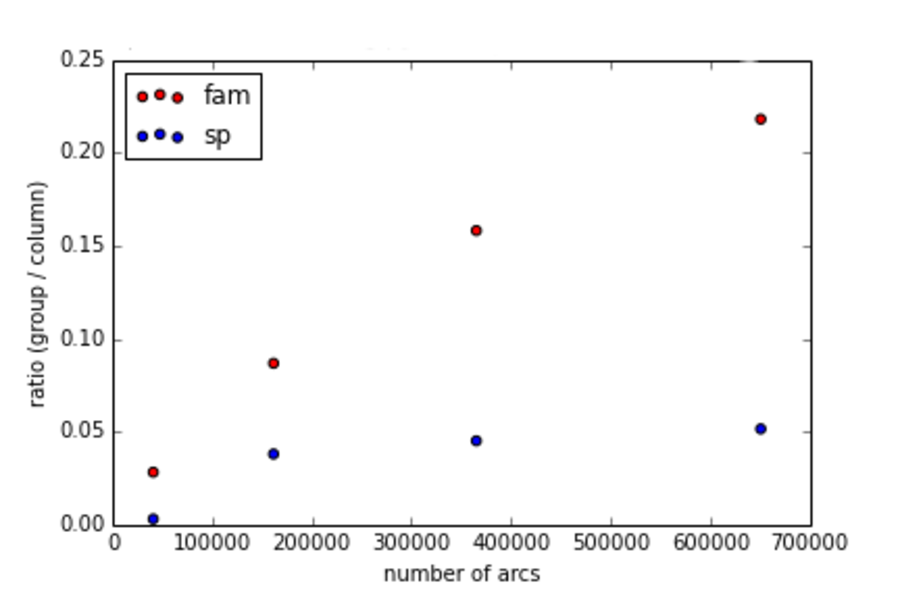
\includegraphics[width=0.85\textwidth]{grp_v_col_ratio.pdf}
    \caption[]{
      \label{fig:col_grp}
      The ratio of group-base d queries to column-based queries as a function of
      problem size. A lower ratio indicates a faster process time for the group
      strategy over the column strategy.}
  \end{center}
\end{figure}

As can be seen, the group-based strategy performs quite well, almost an order of
magnitude better than the column-based strategy. Furthermore, species operations
are shown to have a much larger speedup relative to family operations. This is
due to the fact that at the time of this analysis, solution values were stored
\textit{only if} they were nonzero. When read, a datastructure must be allocated
and populated for each non-zero index rather than simply copying a block on data
on disc. The writing of family-based solution values has since been updated to
also write zero values to avoid this issue.

For the purposes of this study, the dataset-group pivot served the required
purpose. Postprocessing now performs satisfactorily for the operations needed
and the database sizes experienced. However, if future performance issues arise,
other strategies may be investigated. Perhaps the most fruitful of these will be
returning to the single datatset layout and using PyTable's indexing feature. 

\subsection{Implementation}

Cyclopts defines abstract application programming interfaces (APIs) for both
families and species in the \code{ProblemFamily} and \code{ProblemSpecies}
classes, respectively. While many parts of an API are related to the workflow
discussed in \S \ref{method:tools:struc}, others are related to the persistence
mechanisms discussed in \S \ref{method:tools:hdf5}. The full API is described in
detail in the Cyclopts documentation \cite{cyclopts}. The \code{ExchangeFamily}
class implements a concrete, resource-exchange-specific \code{ProblemFamily}
interface. The \code{StructuredRequest} class implements a concrete,
front-end-exchange interface of the \code{ProblemSpecies} class. Similarly, the
\code{StructuredSupply} implements a back-end interface to the class.

Given a point in parameter space, both the \code{StructuredSupply} and
\code{StructuredRequest} generate an instance of an \code{ExchangeGraph} per the
rules described in \S \ref{method:setup}. Cyclopts is nominally written in
Python and Cyclus is written in C++. In order to construct objects that can
interact with Cyclus, an interoperability layer is required. 

A series of C++ wrapper objects, namely arc, node, and group objects, are
defined which mirror the constituents of an \code{ExchangeGraph}, as described
in \S \ref{abm:dre:impl}. These objects are then translated into Cython \cite{}
by use of the XDress software package \cite{xdress}. Python can directly call
into Cython libraries, similarly, Cython can directly call C and C++
libraries. Therefore, a interoperability layer is established.

\subsubsection{Solvers and Performance Timing}

Once an instance of an \code{ExchangeGraph} has been generated, it can be
solved. Cyclopts supports three types of solvers: CoinCLP, CoinCBC, and the
\code{GreedySolver}, an implementation of the Greedy Hueristic in Cyclus. If
either the Greedy or CBC solvers are invoked, an appropriate instance of a
\code{ExchangeSolver} is constructed with the \textit{exclusive orders} flag
turned on. If the CLP solve is invoked, an associated \code{ExchangeSolver}
instance is constructed with the \textit{exclusive orders} flag turned off. In
short, CBC and Greedy solvers solves the MILP formulation of the NFCTP, and the
CLP solver solves the LP formulation.

Given an instance of an \code{ExchangeGraph} and \code{ExchangeSolver}, the
\code{Solve} method of the \code{ExchangeSolver} is invoked. Before and after
the \code{Solve} function call, the \code{CoinCpuTime} function is called and
the result is stored. The difference between the two resulting values is
recorded as the time required to determing a solution. The implementation of the
\code{CoinCpuTime} function is open and easily available \cite{}. It simply adds
the seconds and microseconds fields of the \code{ru_utime} structure populated
by the standard UNIX \code{getrusage} function.

\subsection{High Throughput Computing}\label{method:tools:htc}

Cyclopts can be executed locally using the \code{cyclopts exec} CLI described
in \label{method:tools:cli}. When exploring a large parameter space, of which
each point can generate a large number of unique instances, local execution on a
single machine is insufficient. In order to overcome this limitation, support
for Condor-based systems has been implemented in Cyclopts and available using
the \code{cyclopts condor-submit} CLI. Condor \cite{condor-practice} is a high
throughput computing (HTC) framework that supports sophisticated job scheduling
over a very large, distributed network of individual and clustered computers.

HPC systems are ideal for analysis in which many independent executions may be
performed independently. Upon completion, the resulsts may be aggregated and
analyzed. The resource exchange use case fits such a design specification with a
single caveat: because it is a first-of-a-kind, performance analysis, timing
results are crucial. Therefore, the systems on which instances are executed must
be equivalent in order to compare different timing results. Support is provided
in Cyclopts for identifying execute nodes that conform to a series of
architecture and relate constraints in order to enforce this limitation.

\subsubsection{Remote Execution and Operation}

In order to efficiently schedule a large number of optimization problems, the
WorkQueue framework \cite{bui_work_2011} is utilized. WorkQueue is a
Condor-aware master-worker implementation. A master process exists at some
location and is schedules jobs to be run. Workers, in the form of persistent
Condor jobs, ask the master for the next job to be run after a previous job has
been completed.

Cyclopts launches a master process that requires a series of execute nodes to
target, a problem instance database, and a list of solvers to execute on each
instance. A copy of the instance database is sent to every targeted execute
node. Note that an execute node may have many execution threads, each of which
can be used to execute instances individually. The master manages an instance
queue. Each worker is given an initial instance to execute. Upon completion, a
worker will request a new instance of the master. The full set of instances in a
database are thusly efficiently executed.

\subsubsection{Packaging and Environment}

A common issue in remote execution envrionments is package dependency. When
access to an execution node is provided, a user must assume that only the barest
of environments exist. For example, if a user is provided an Ubuntu-based
execution node, the user generally must assume that it is a fresh Ubuntu
installation. Accordingly, package management in a highly distributed,
heterogenous envrionment is a difficult problem.

Luckily, solutions exist for distributed package management. Cyclopts utilizes
the Code, Data, and Environment (CDE) \cite{cde} tool to manage its execution
environment. CDE provides a virtualized environment based on the local execution
of a command. Using CDE with the given command, all libraries and utilies used
during the execution of the command process are monitored. Upon process exit,
every object in the filesystem that was invoked is copied into a virtual
environment. That virtual environment can then be packaged and distributed. Upon
landing on a foreign system, a user can enter the CDE enviornment and execute
the supported command.

Cyclopts provides a CLI, \code{cyclopts cde}, that will package Cyclopts itself
into a virtual environment and ship the environment to a Condor submit node. As
part of the Cyclopts Condor job execution, the CDE environment is copied to each
submit node. It is thus easy to incorporate changes in a local copy of Cyclopts
to the corresponding remote execution.

\subsection{Command Line Interface}\label{method:tools:cli}

Cyclopts provides a rich command line interface (CLI) for instance generation,
local execution, and remote execution. The CLI includes a number of useful
utilities, however this section will only present those required for running the
full Cyclopts workflow, both local and remote. The full set of CLI options is
presented in Listing \ref{lst:loptshlep}.

\lstinputlisting[
  style=BashOutputStyle,
  keywordstyle=\ttfamily,
  caption={All available Cyclopts CLI options (the result of \code{cyclopts -h}).}, 
  label=lst:loptshlep]{./chapters/3-method/listings/help}

When working locally, the primary workflow is \code{cyclopts convert}, followed
by \code{cyclopts exec}, finishing with \code{cyclopts pp}. \code{cyclopts
  convert} converts a user-provided definition of a parameter space into an
instance database. \code{cyclopts exec} then executes some of all of those
instances, resulting in a solution database. Finally, \code{cyclopts pp} post
processes the instance and solution data. The options for each are described in
Listings \ref{lst:loptsconvert}, \ref{lst:loptsexec}, and \ref{lst:loptspp},
respectively.

\lstinputlisting[
  style=BashOutputStyle,
  keywordstyle=\ttfamily,
  caption={CLI options for \code{cyclopts convert}.}, 
  label=lst:loptsconvert]{./chapters/3-method/listings/convert}

\lstinputlisting[
  style=BashOutputStyle,
  keywordstyle=\ttfamily,
  caption={CLI options for \code{cyclopts exec}.}, 
  label=lst:loptsexec]{./chapters/3-method/listings/exec}

\lstinputlisting[
  style=BashOutputStyle,
  keywordstyle=\ttfamily,
  caption={CLI options for \code{cyclopts pp}.}, 
  label=lst:loptspp]{./chapters/3-method/listings/pp}

In order to execute Cyclopts on a Condor system, the submit node must contain
the Cyclopts environment. That operation is supported by the \code{cyclopts cde}
CLI, presented in Listing \ref{lst:loptscde}. A job, the input of which is an
instance database, can be submitted using \code{cyclopts condor-submit}. Upon
completion, results can be collected with \code{cyclopts condor-collect}. The
arguments for both are shown in Listings \ref{lst:loptscondor-submit} and
\ref{lst:loptscondor-collect}.

\lstinputlisting[
  style=BashOutputStyle,
  keywordstyle=\ttfamily,
  caption={CLI options for \code{cyclopts cde}.}, 
  label=lst:loptscde]{./chapters/3-method/listings/cde}

\lstinputlisting[
  style=BashOutputStyle,
  keywordstyle=\ttfamily,
  caption={CLI options for \code{cyclopts condor-submit}.}, 
  label=lst:loptscondor-submit]{./chapters/3-method/listings/condor-submit}

\lstinputlisting[
  style=BashOutputStyle,
  keywordstyle=\ttfamily,
  caption={CLI options for \code{cyclopts condor-collect}.}, 
  label=lst:loptscondor-collect]{./chapters/3-method/listings/condor-collect}
